\documentclass[11pt,twocolumn,twoside]{IEEEtran}
\usepackage{amsmath}
\usepackage[pdftex]{epsfig}
\usepackage{amsfonts}
\usepackage{amssymb}
\usepackage{fancyhdr}
\usepackage{url}
\include{graphicsx}

\pagestyle{fancy}
%\renewcommand{\headrulewidth}{0pt}
\renewcommand{\footrulewidth}{0pt}
\rhead{
\includegraphics[height=0.6in]{cilogo.png}}
\fancyhead[LO]{\sc sci-wms\ldots} % shorter form of title to fit in space
\fancyhead[LE]{\sc Mayer, McKenna, Knee} % author list or et al., to fit in space
\chead{}
\cfoot{}

\begin{document}
\title{\vspace{0.2in}\sc sci-wms:A python-based Web Map Service for Visualizing Geospatial data}

\author{Brandon A. Mayer$^{1,2}$, Brian McKenna$^{2}$, Kelly Knee$^{2}$\thanks{Brown University School Of Engineering$^{1}$, RPS-Applied Science Associates, South Kingston RI$^{2}$, Brandon\_Mayer@brown.edu, BMcKenna@asascience.com, KKnee@asascience.com}}

\maketitle
\thispagestyle{fancy}

\begin{abstract}
This paper outlines the implementation and technology stack for
visualizing geo-registered meterological forecasting data using
sci-wms~\cite{wms14}.\footnote{https://github.com/asascience-open/sci-wms}
Specifically, we consider a use case in which sci-wms was used as a
back end to create a custom web-portal for visualizing externally
hosted data sets indexed by the National Geophysical Data Center
(NGDC)~\cite{luettich13}~\cite{luettich12}. By separating model topology and variable values, sci-wms is
able to serve custom generated content for a diverse range of models,
including SELFE, FVCOM, SLOSH and ADCIRC in real time to many
simultaneous clients in response to standard http GET requests.
\end{abstract}

\section{Motivation}
The ubiquity of computing hardware, interconnected by the
world-wide-web, has lead to the proliferation of both meterological
data and the development of models for the interpretation of said
data. As scientists continue to refine and develop models to simulate
and analyze storm data, an simple and efficient work flow for model
aggregation and comparison, whether for forecasting purposes or
retrospective model evaluation is essential for streamlining the
scientific process.

sci-wms is a software solution able to visualize meterological
simulations regardless of the underlying methodology by abstracting a
data set into two distinct objects: the simulation topology and
simulation variables. Model topology refers to a geo-referenced set of
geometrical objects which define the positions and connectivity that
variables in the data set may occupy. The types of topologies are just
a numerous as the quantity of standard forecasting models, with some
models able to generate multiple topologies. For example, there are
curvelinear, rectilinear, regular, or unstructured triangular grids
which can be in the planar 2D or volumetric 3D varieties.

\begin{figure}
  \centering
  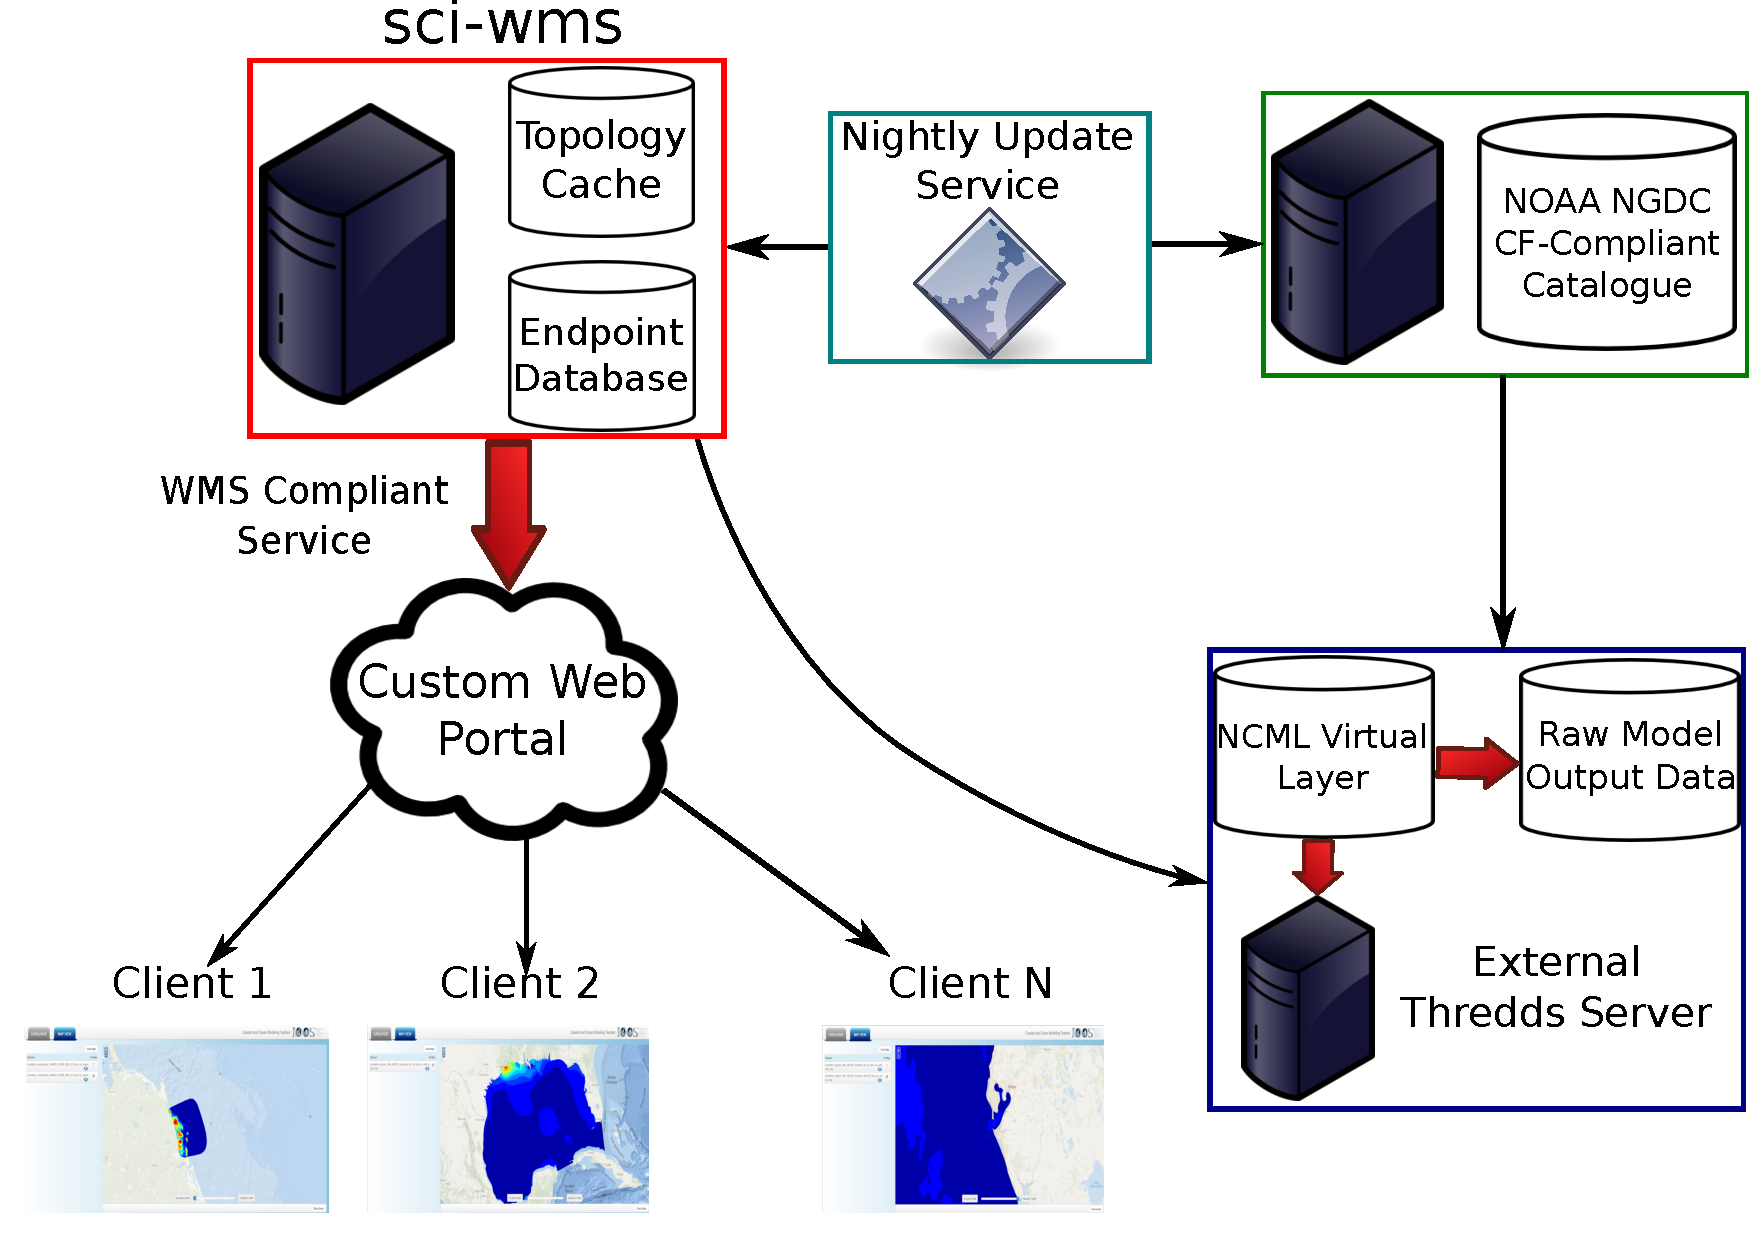
\includegraphics[width=\columnwidth]{./figs/overview.pdf}
  \caption{COMT-SURA deployment of sci-wms for oceanagraphic modeling visualization.}
  \label{fig:overview1}
\end{figure}

\bibliographystyle{ieeetr}
\bibliography{ci_mayer}
%% \bibliography{bibfile,benherzog}

\end{document}
